\chapter{Introduction}

\section{Background and motivation}
On June 30th 2000, nine young men passed away in a crowd crush during a Pearl Jam concert at Roskilde Festival in Denmark \cite{pearl_jam}. An uncontrolled surge, pushing the crowd towards the scene, caused immense pressure on the frontmost concert-goers, thrusting them against the barriers. The high-energy crowd unknowingly trampled the victims, who succumbed under the pressure of the crowd. This incident is unfortunately not the only one of its kind, as crowd crushes continue to occur at mass gatherings around the world.

\section{Problem definition}
\label{sec:problem-definition}

The problem boils down to crowd safety managers being very busy, while having a very important job to do.
\section{Brief history of Fluxense}

Together with two classmates, I founded a startup, Fluxense, in January 2024. Our initial idea was to improve crowd safety at large gatherings with an AI-enabled system that monitors existing CCTV infrastructure to provide automated analyses of crowd behavior. We gained traction quickly, with several large festivals expressing their interest in our proposed product. Development began almost immediatelly, and we held our first prototype test at DTU's Commemoration Day, where we provided a live count of the number of people in the concert hall. The test gave great results, as well as valuable learnings, and became the first of many. The following summer was very busy, as we attended three of Denmarks largest music festivals -- Copenhell, Roskilde Festival and Smukfest -- to further test and develop our product.

After the summer, we stood at a crossroads. Our collaborations with the different festivals had revealed that each had their own unique requirements, and the value of our product was not as clear-cut as we had initially thought. We feared that crowd safety was not a large enough market for scaling our business, nor that a generalized product would be attractive in the industry. We decided to pivot, and began exploring other markets where our technology could be of use. We gradually moved away from our initial focus on crowd safety, and found business intelligence to be a much larger and lucrative market. Instead of monitoring crowds, our new product would track individual customers in retail stores, transportation hubs, amusemenent parks, and museums. We aimed to provide insights into places/products of interest, dwell times, conversion rate, footfall analysis, etc., to help businesses optimize their operations.

As the autumn progressed, we began securing new collaborations in our target industry, and our value proposition became clearer. One important thing had been lost in the process, however: our motivation. We had started Fluxense with the goal of improving crowd safety at music festivals, as it was a mission we shared a passion for. Our new focus on business intelligence made sense fiscally, but didn't evoke the same feeling of purpose. Fluxense ended up dissolving in the winter of 2024/25, as we couldn't see ourselves in the startup's new reality, and struggled to find a common vision.

\section{Scope and limitations}

This thesis continues where Fluxense left off before the pivot. Rather than focusing on a scalable business model, the goal is to design and develop a product that can assist crowd safety managers in their work. This project is specifically tailored to Roskilde Festival

\section{Mission statement}

\section{Thesis structure}

In their book, \textit{Design Science}, Hubka and Eder characterize the design process as intuitive, iterative, innovative, unpredictable and reflective \cite{hubka_eder}.

Process needs to organized. (citation?)

Blah blah, following product design methodology / frameworks. Many frameworks exist

\subsection{Comparison of frameworks}
\vspace{2em}
\begin{figure}[H]
  \centering
  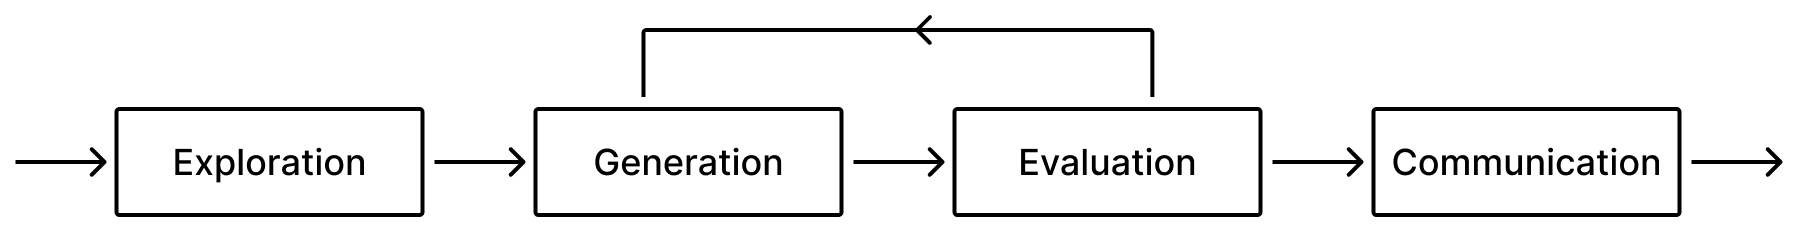
\includegraphics[width=14cm]{Pictures/Figures/cross.png}
  \caption{Cross' four-stage model of the design process}
  \label{fig:cross}
\end{figure}

Cross \cite{cross} proposes likely the most simplistic, yet well-known framework: a four-stage model comprised of \textit{exploration}, \textit{generation}, \textit{evaluation} and \textit{communication} (Figure \ref{fig:cross}). Cross describes this type of modal as descriptive, as it merely attempts to model the conventional, heuristic design process. More detailed models of this type exist, such as French's \cite{french} "anatomy of design," (Figure x) detailing four stages, most distinctly underlining the problem analysis and definition, as conducted in section \ref{sec:problem-definition}. According to Cross, these models differ from prescriptive models, which offer a more systematic procedure, as well an emphasis on analyzing and understanding the design problem before generating solution concepts. Perhaps the most well-known of these is offered by Pahl et. al \cite{pahl_beitz}, and is based on the following design stages: \textit{clarification of the task}, \textit{conceptual design}, \textit{embodiment design}, and \textit{detail design}. Combining the aforementioned models, Ulrich and Eppinger present a rather comprehensive framework. Their process is based on the following stages: \textit{concept development}, \textit{system-level design}, \textit{detail design}, and \textit{testing and refinement} \cite{ulrich_eppinger}.

These frameworks provide varying degrees of structure and granularity to the design/development process, but all share the commonality of being highly engineering-focused. In engineering a physical product, a rigid, structured process is often necessary as each iteration must be designed, manufactured and tested. This is costly, both in effort and material costs. Therefore, the design and development process are divded and sequential. Software, on the other hand, is much more flexible, with iterations being a magnitude faster and cheaper to develop. This demonstrates a need for adapting the design/development process to the context of the product being developed. Conveniently, Ulrich and Eppinger present a multitude of adaptations to their framework, including what they refer to as "Quick-Build Products" and "Digital Products." Here the \textit{detail design} and \textit{testing and refinement} stages are omitted, and replaced with a cyclical design-build-test process. Whereas the linear, rigid processes described previously are labelled as "waterfall methods", this iterative process is most often referred to as \textit{agile development}.

Agile development has many benefits in contrast to the waterfall approach, especially in the context of software development. As mentioned previously, the waterfall approach is ideal for engineering projects where prototyping is costly. When the cost of protoyping is negligible, however, agile grants the flexibility to iterate quickly, and adapt to evolving requirements. Design and development are sequential in a waterfall model; here they are heavily intertwined. A strong example as this, as well as being the most popular implementation of agile development, is \textit{Scrum}. Scrum defines the following stages: \textit{sprint planning}, \textit{daily stand-up}, \textit{sprint review}, and \textit{sprint retrospective}, with a sprint typically lasting 2-4 weeks \cite{scrum}.

Blah blah blah scrum is good for large teams, not ideal at this scale.

\subsection{Design and development methodology}